\chapter[Transferência e extrapolação]{Transferência Espacial e Temporal, Extrapolação, MESS e MOP}

\begin{objetivos}
	Ao final desta unidade, o estudante deverá compreender os desafios da transferência espacial e temporal em SDM; diferenciar interpolação e extrapolação ambiental; calcular mapas MESS e MOP; identificar áreas futuras fora do domínio ambiental de calibração; avaliar riscos de extrapolação nas projeções climáticas de \textit{Dinizia excelsa}; e interpretar mapas futuros considerando incerteza ambiental.
\end{objetivos}

\section{Introdução}

Modelos de distribuição de espécies são frequentemente calibrados sob condições ambientais atuais e depois transferidos para outros espaços ou períodos, como cenários climáticos futuros, períodos paleoclimáticos ou regiões geográficas distintas. Essa transferência é uma das aplicações mais importantes de SDM, mas também uma das mais sensíveis a erros \parencite{peterson2011,araujo2012,yates2018transferability,zurell2020benchmarking}.

Quando um modelo é projetado para condições ambientais semelhantes às usadas na calibração, estamos diante de uma situação de interpolação ambiental. Por outro lado, quando o modelo é aplicado a condições ambientais fora do intervalo conhecido, ocorre extrapolação. Nesses casos, as predições podem ser estatisticamente possíveis, mas ecologicamente frágeis.

\begin{conceito}[title={\faBook\quad Interpolação versus extrapolação}]
	Interpolação ocorre quando o modelo é projetado para combinações ambientais semelhantes às observadas na calibração. Extrapolação ocorre quando o modelo é aplicado a valores ou combinações ambientais não representadas nos dados usados para ajustar o modelo.
\end{conceito}

\section{Transferência espacial e temporal}

A transferência espacial ocorre quando um modelo calibrado em uma região é aplicado a outra região. A transferência temporal ocorre quando um modelo calibrado no presente é aplicado ao passado ou futuro. Em ambos os casos, a confiabilidade depende da similaridade ambiental entre calibração e projeção.

\begin{atencao}[title={\faExclamationTriangle\quad Projeções futuras exigem diagnóstico de extrapolação}]
	Mapas futuros de adequabilidade não devem ser interpretados isoladamente. Eles precisam ser avaliados junto com mapas de similaridade ambiental, como MESS e MOP.
\end{atencao}

\section{MESS: Multivariate Environmental Similarity Surface}

O MESS avalia, para cada célula projetada, se seus valores ambientais estão dentro do intervalo observado na região de calibração. Valores positivos indicam similaridade ambiental; valores negativos indicam extrapolação univariada em pelo menos uma variável.

\rscriptfile{scripts/unidade14/01_estrutura_pastas.R}

\rscriptfile{scripts/unidade14/02_calcular_mess_futuro.R}

\begin{figure}[H]
	\centering
	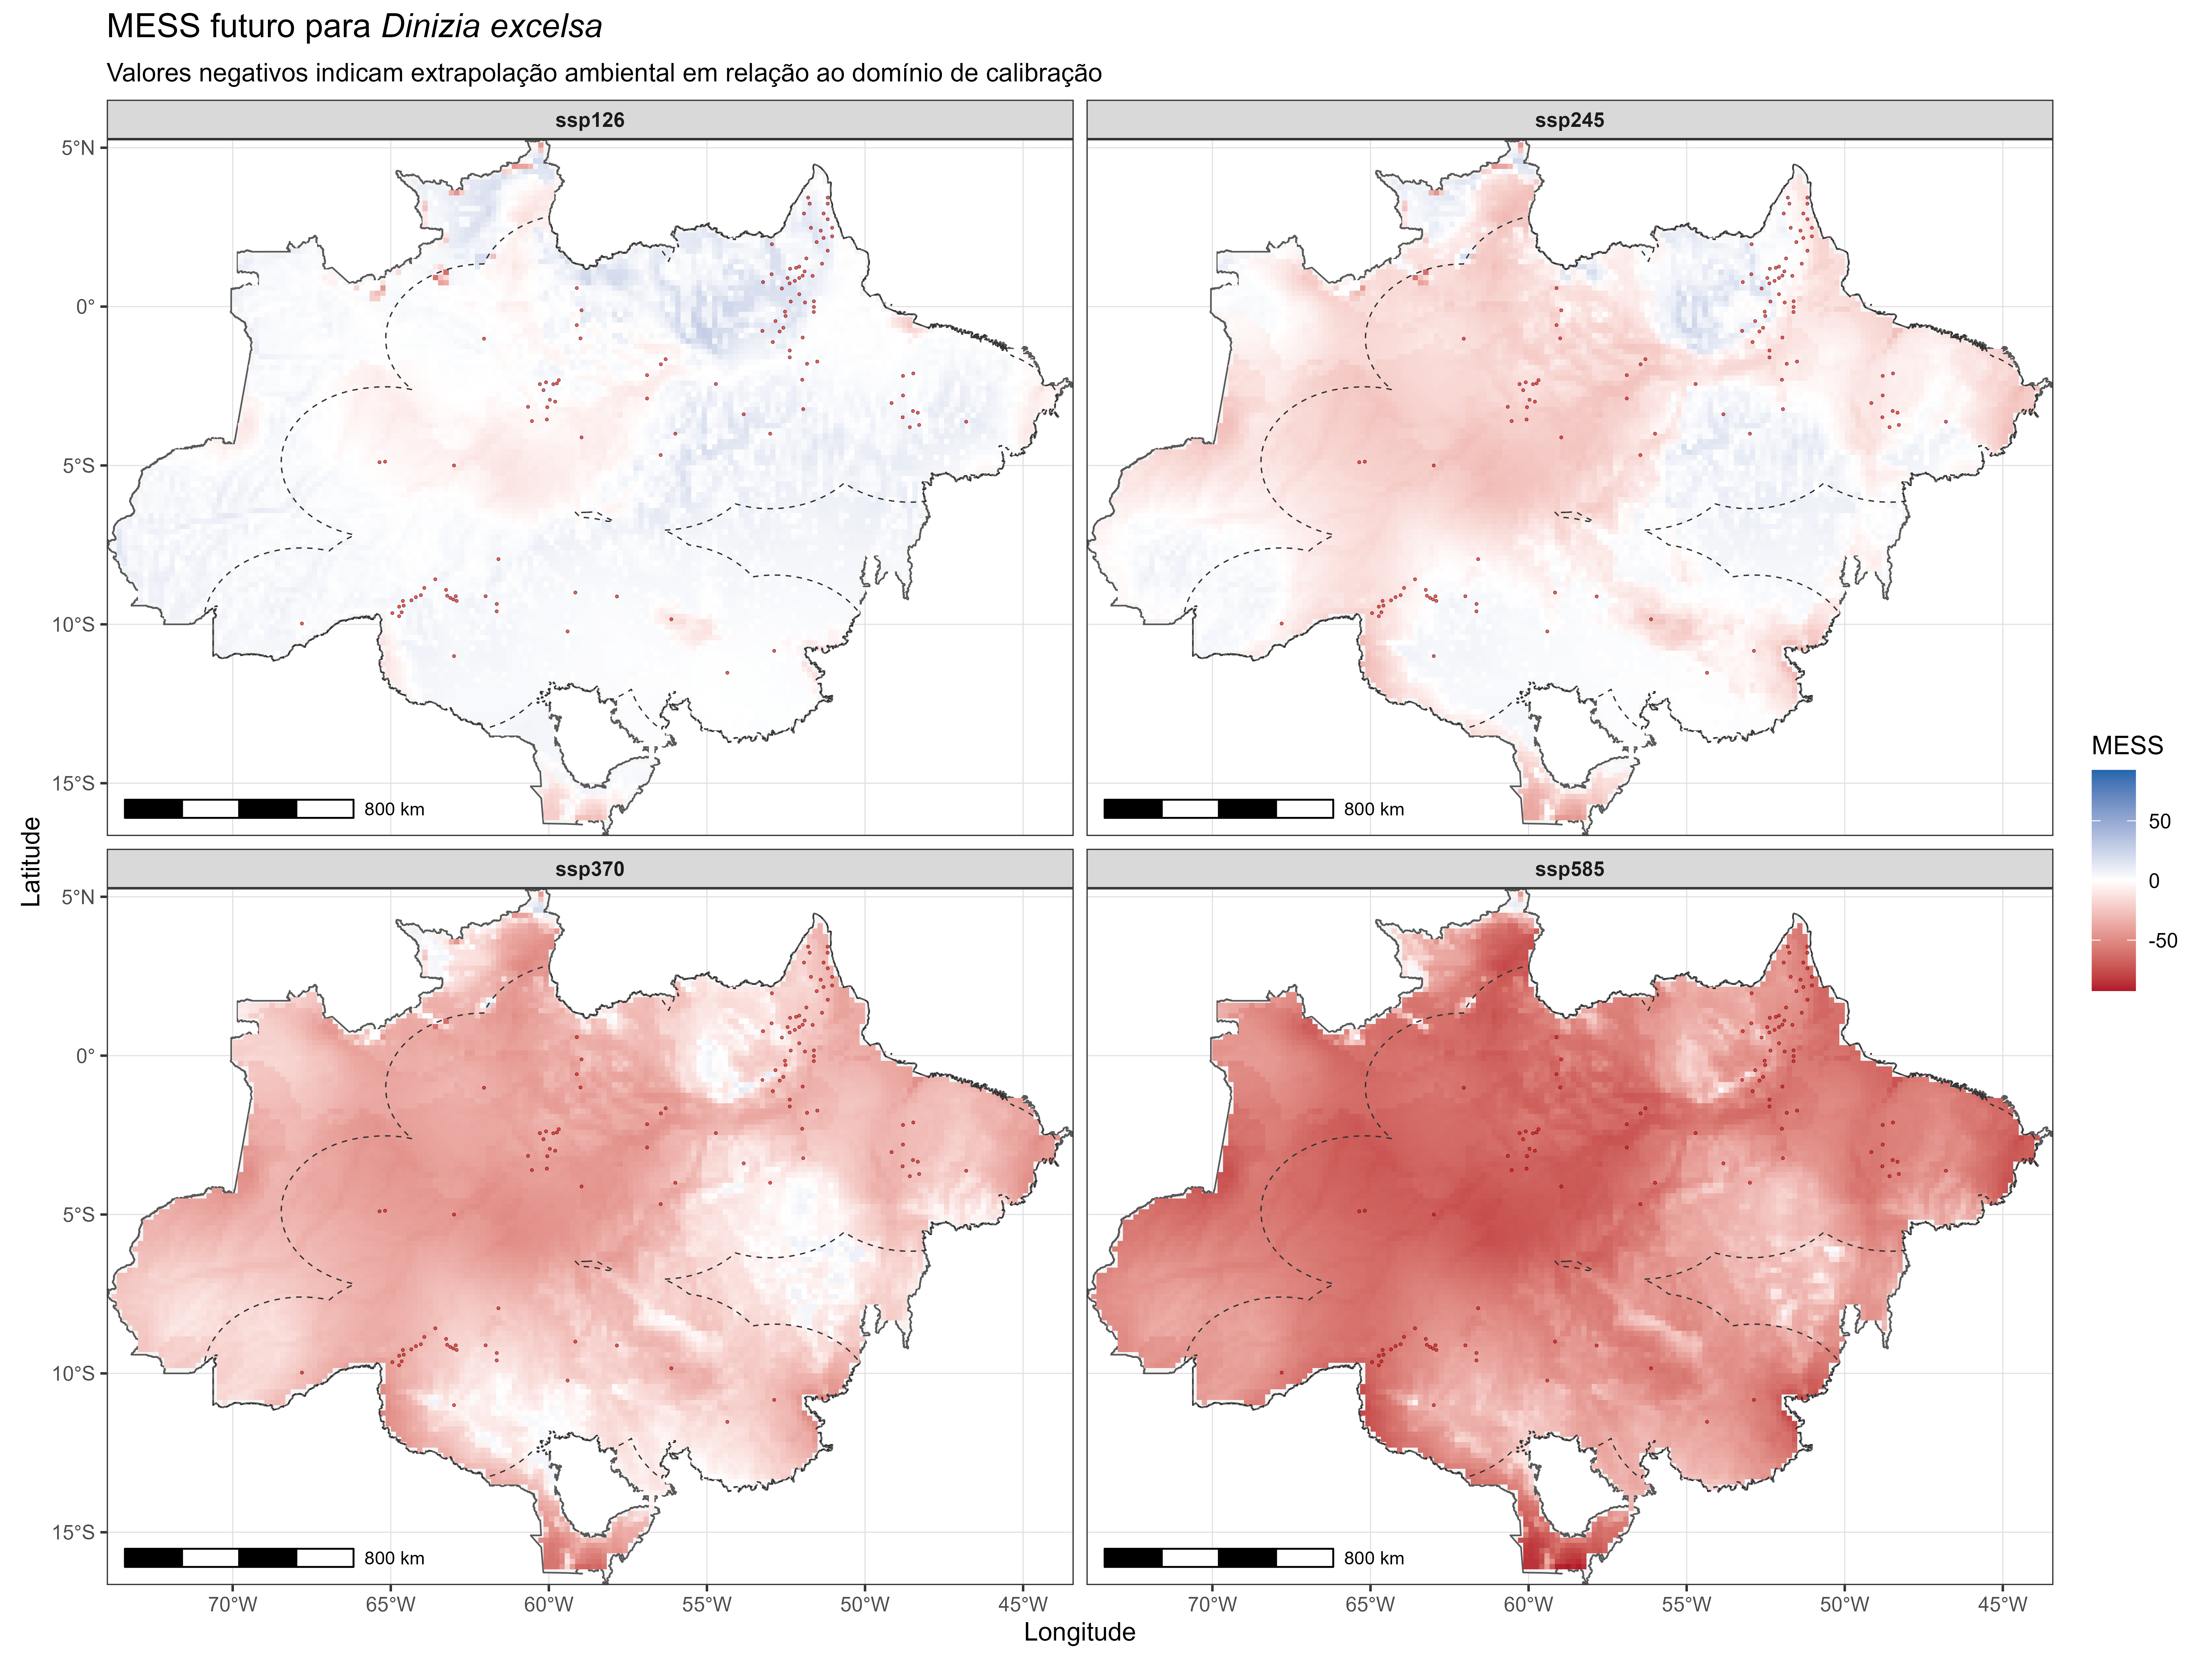
\includegraphics[width=0.96\textwidth]{figuras/unidade14/unidade14_mess_cenarios.png}
	\caption{Mapas MESS para os cenários futuros de \textit{Dinizia excelsa}. Valores negativos indicam extrapolação ambiental em relação ao domínio de calibração.}
	\label{fig:unidade14_mess}
\end{figure}

\section{Variável limitante no MESS}

Além do valor de similaridade, é possível identificar qual variável ambiental é responsável pela maior extrapolação em cada célula. Essa análise ajuda a interpretar se a incerteza futura decorre principalmente de temperatura, precipitação ou sazonalidade.

\rscriptfile{scripts/unidade14/03_variavel_limitante_mess.R}

\begin{figure}[H]
	\centering
	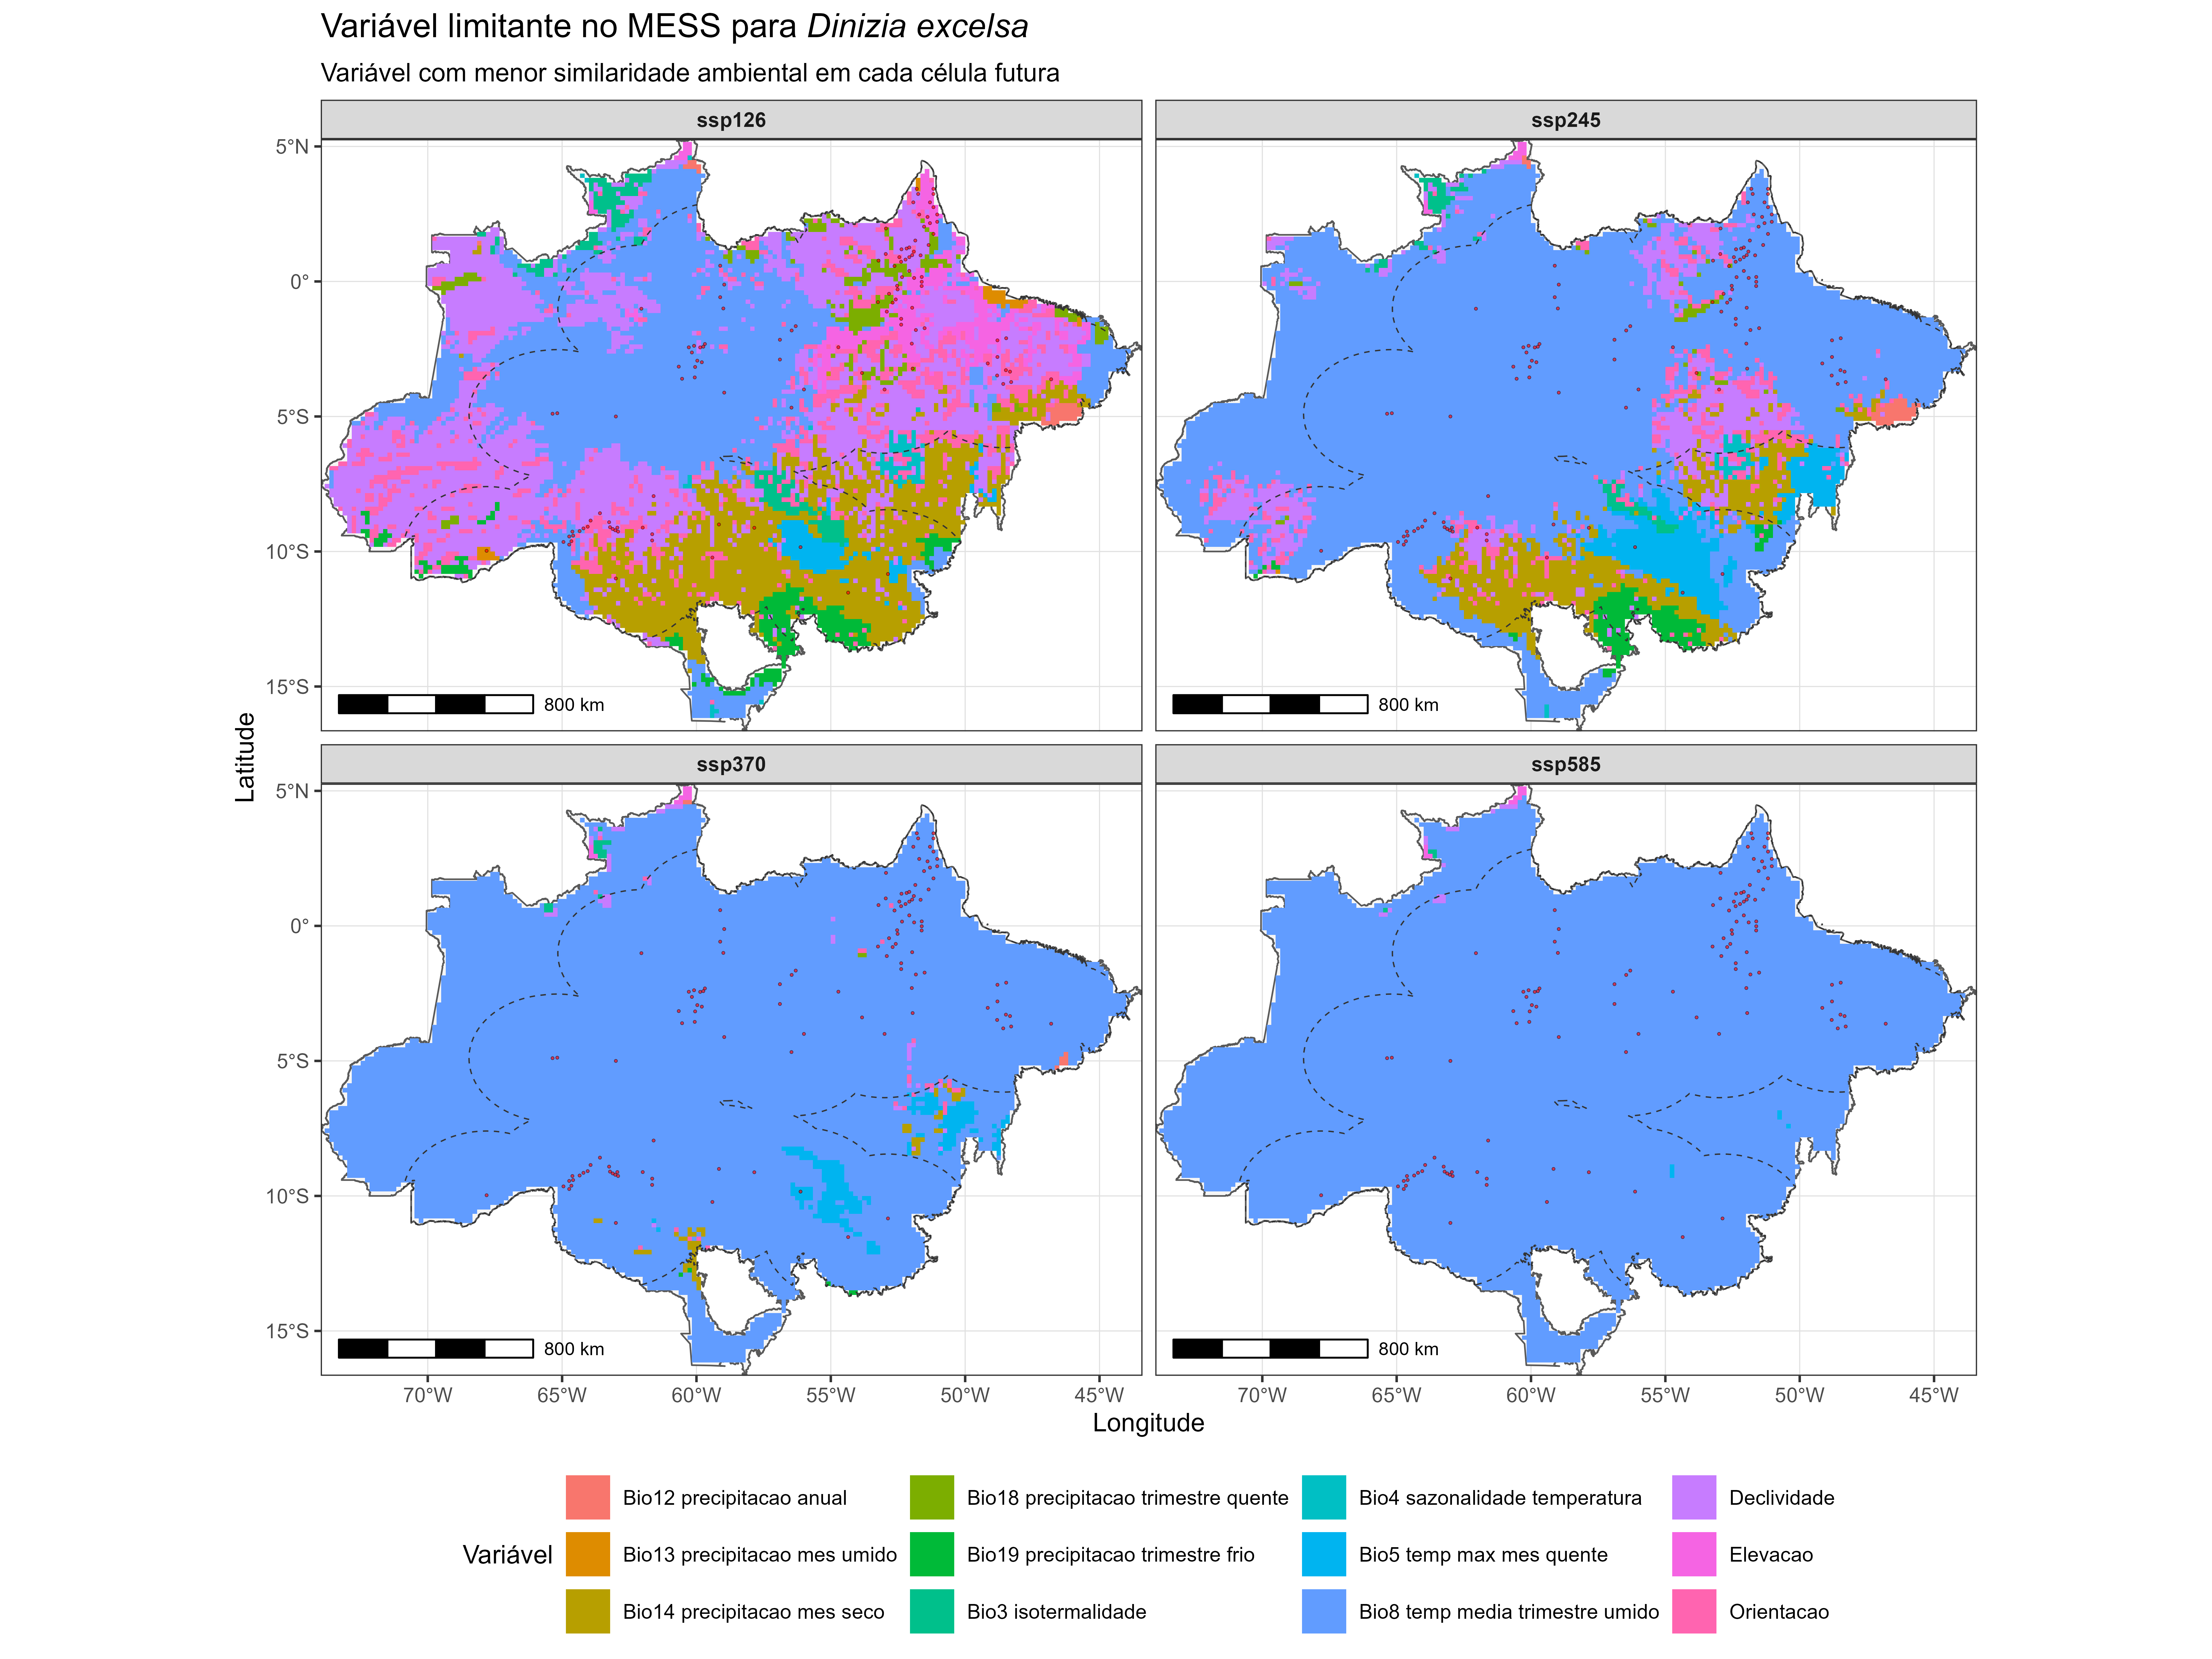
\includegraphics[width=0.96\textwidth]{figuras/unidade14/unidade14_variavel_limitante_mess.png}
	\caption{Variável ambiental mais limitante no diagnóstico MESS para os cenários futuros.}
	\label{fig:unidade14_limitante}
\end{figure}

\section{MOP: Mobility-Oriented Parity}

O MOP avalia a similaridade multivariada entre ambientes de calibração e projeção, considerando a distância ambiental entre células. Diferentemente do MESS, que avalia limites univariados, o MOP considera combinações ambientais multivariadas e identifica áreas ambientalmente não análogas \parencite{owens2013constraints}.

\rscriptfile{scripts/unidade14/04_calcular_mop_futuro.R}

\begin{figure}[H]
	\centering
	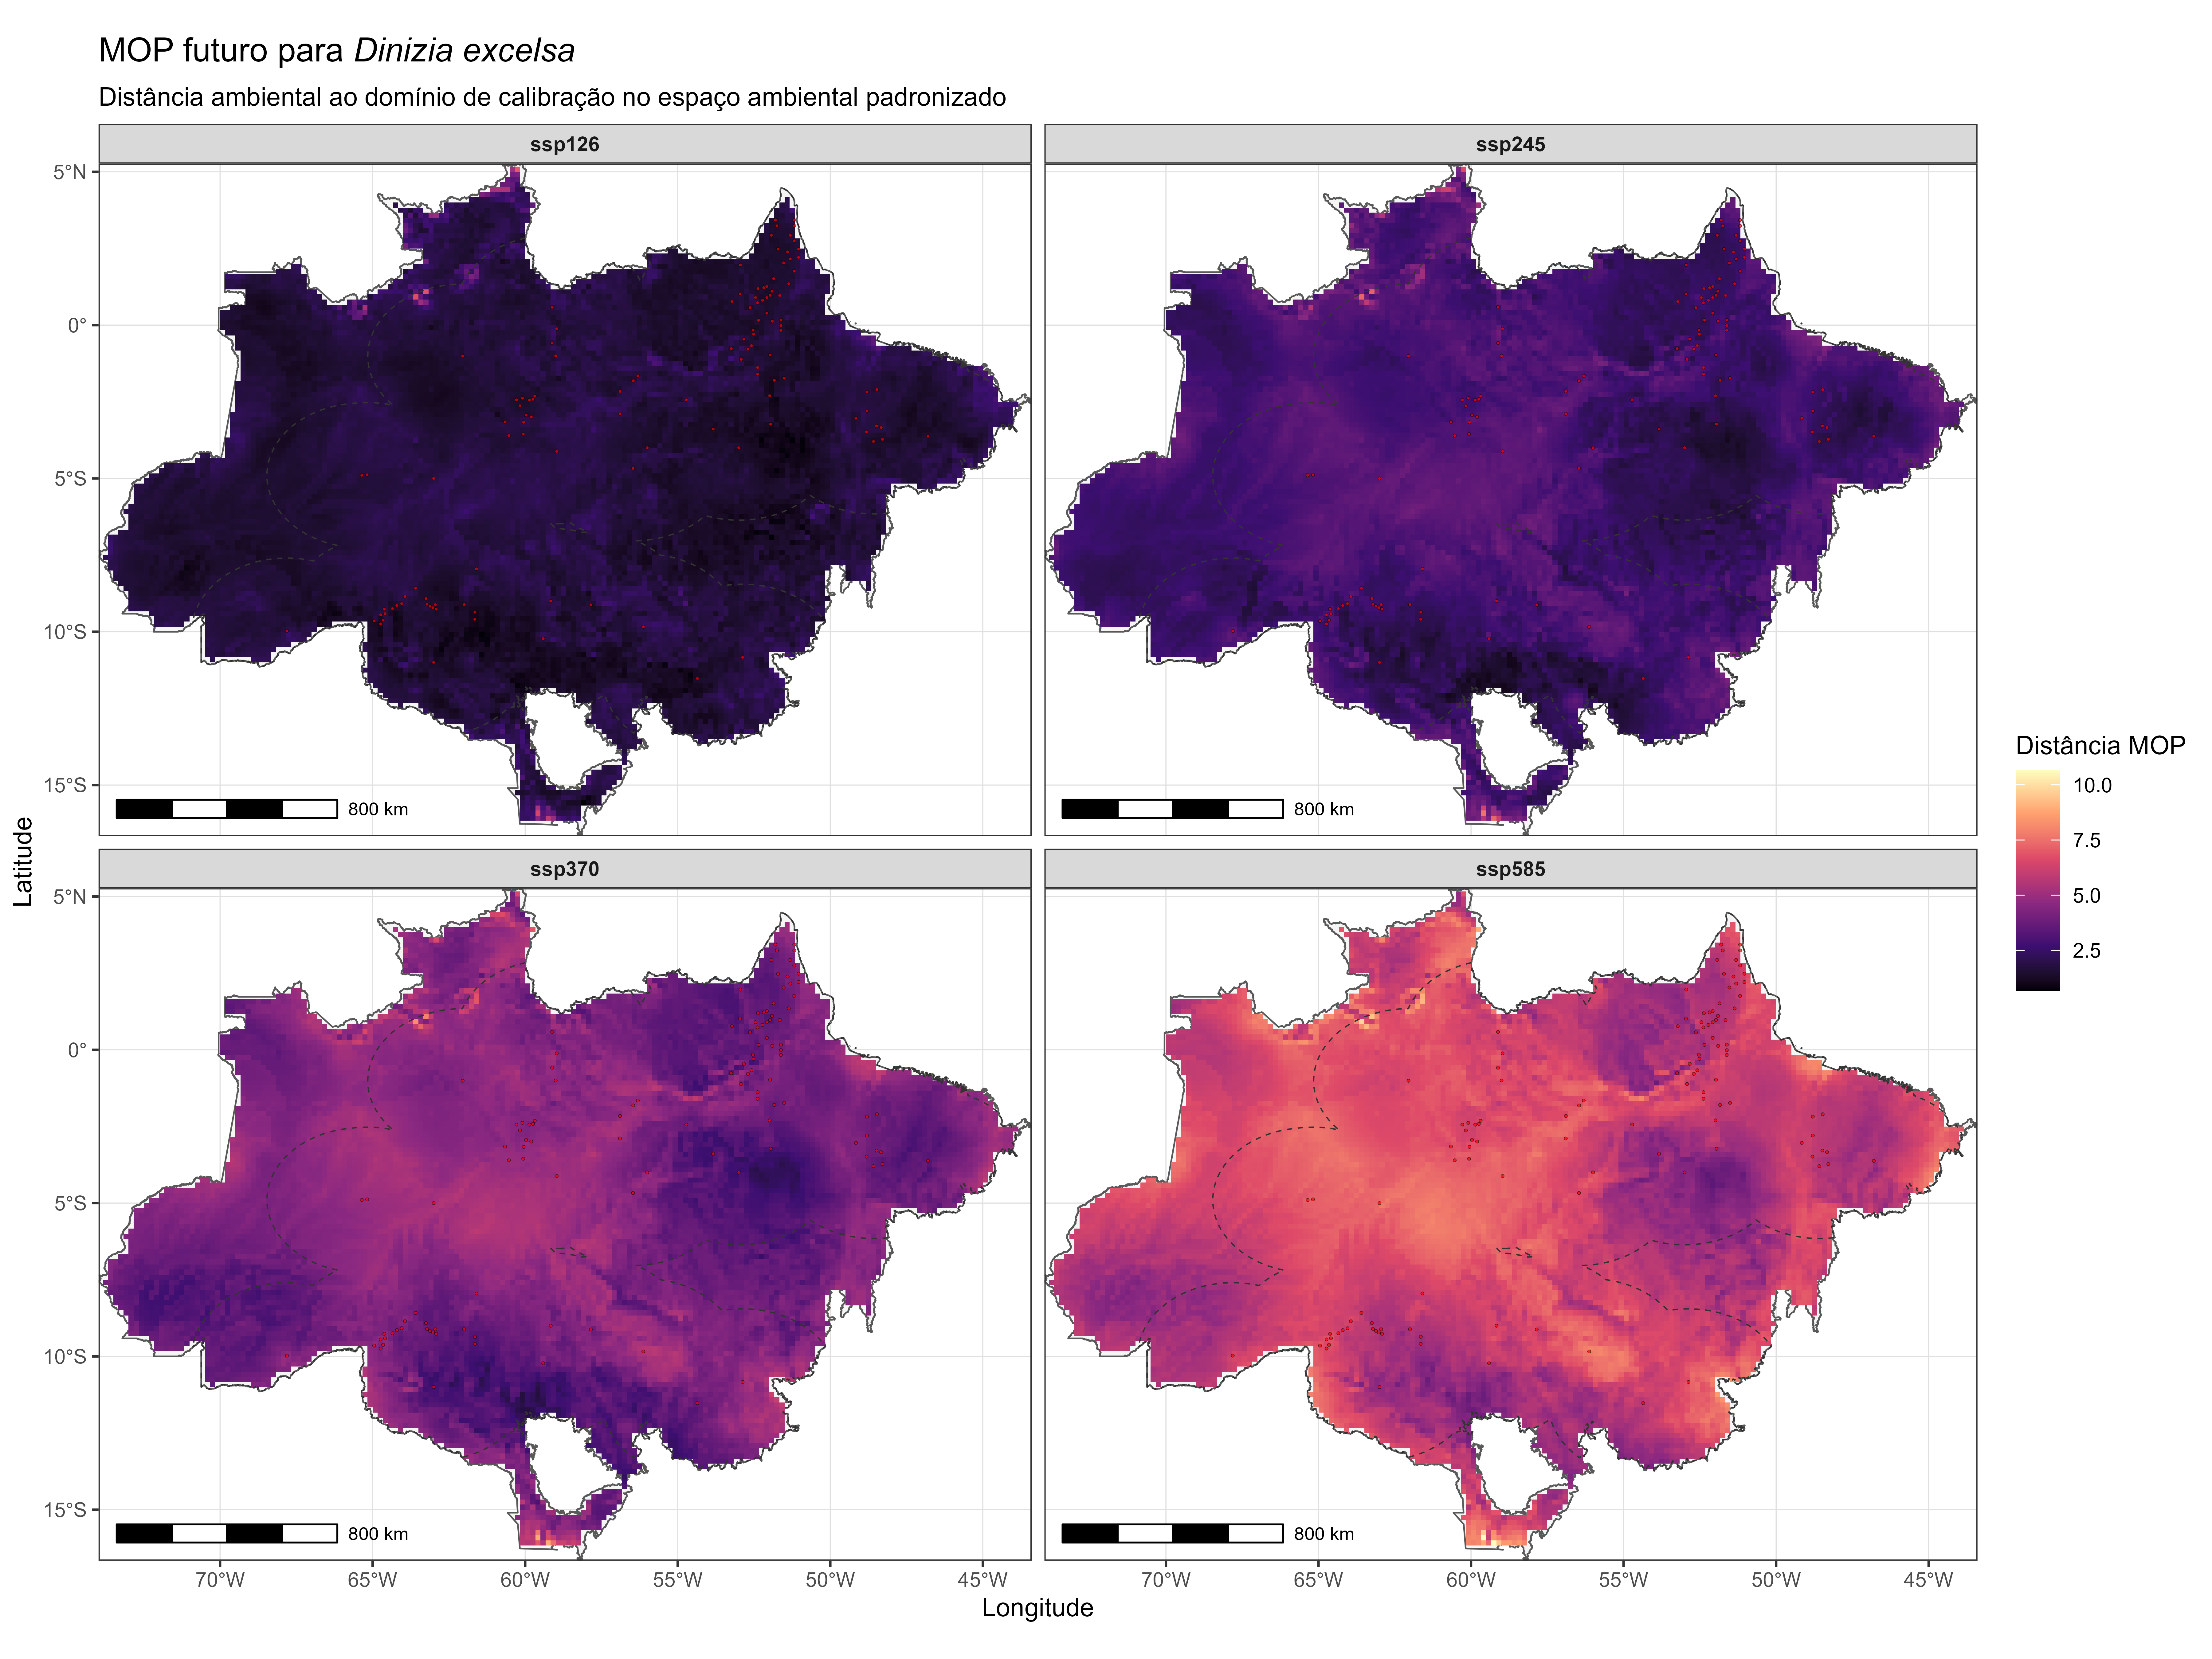
\includegraphics[width=0.96\textwidth]{figuras/unidade14/unidade14_mop_cenarios.png}
	\caption{Mapas MOP simplificados para os cenários futuros. Valores mais altos indicam maior distância ambiental em relação ao domínio de calibração.}
	\label{fig:unidade14_mop}
\end{figure}

\section{Adequabilidade sob extrapolação}

Nesta etapa, os mapas de adequabilidade futura são combinados com os mapas MESS e MOP. O objetivo é identificar áreas projetadas como adequadas, mas sob condições extrapolativas.

\rscriptfile{scripts/unidade14/05_adequabilidade_extrapolacao.R}

\begin{figure}[H]
	\centering
	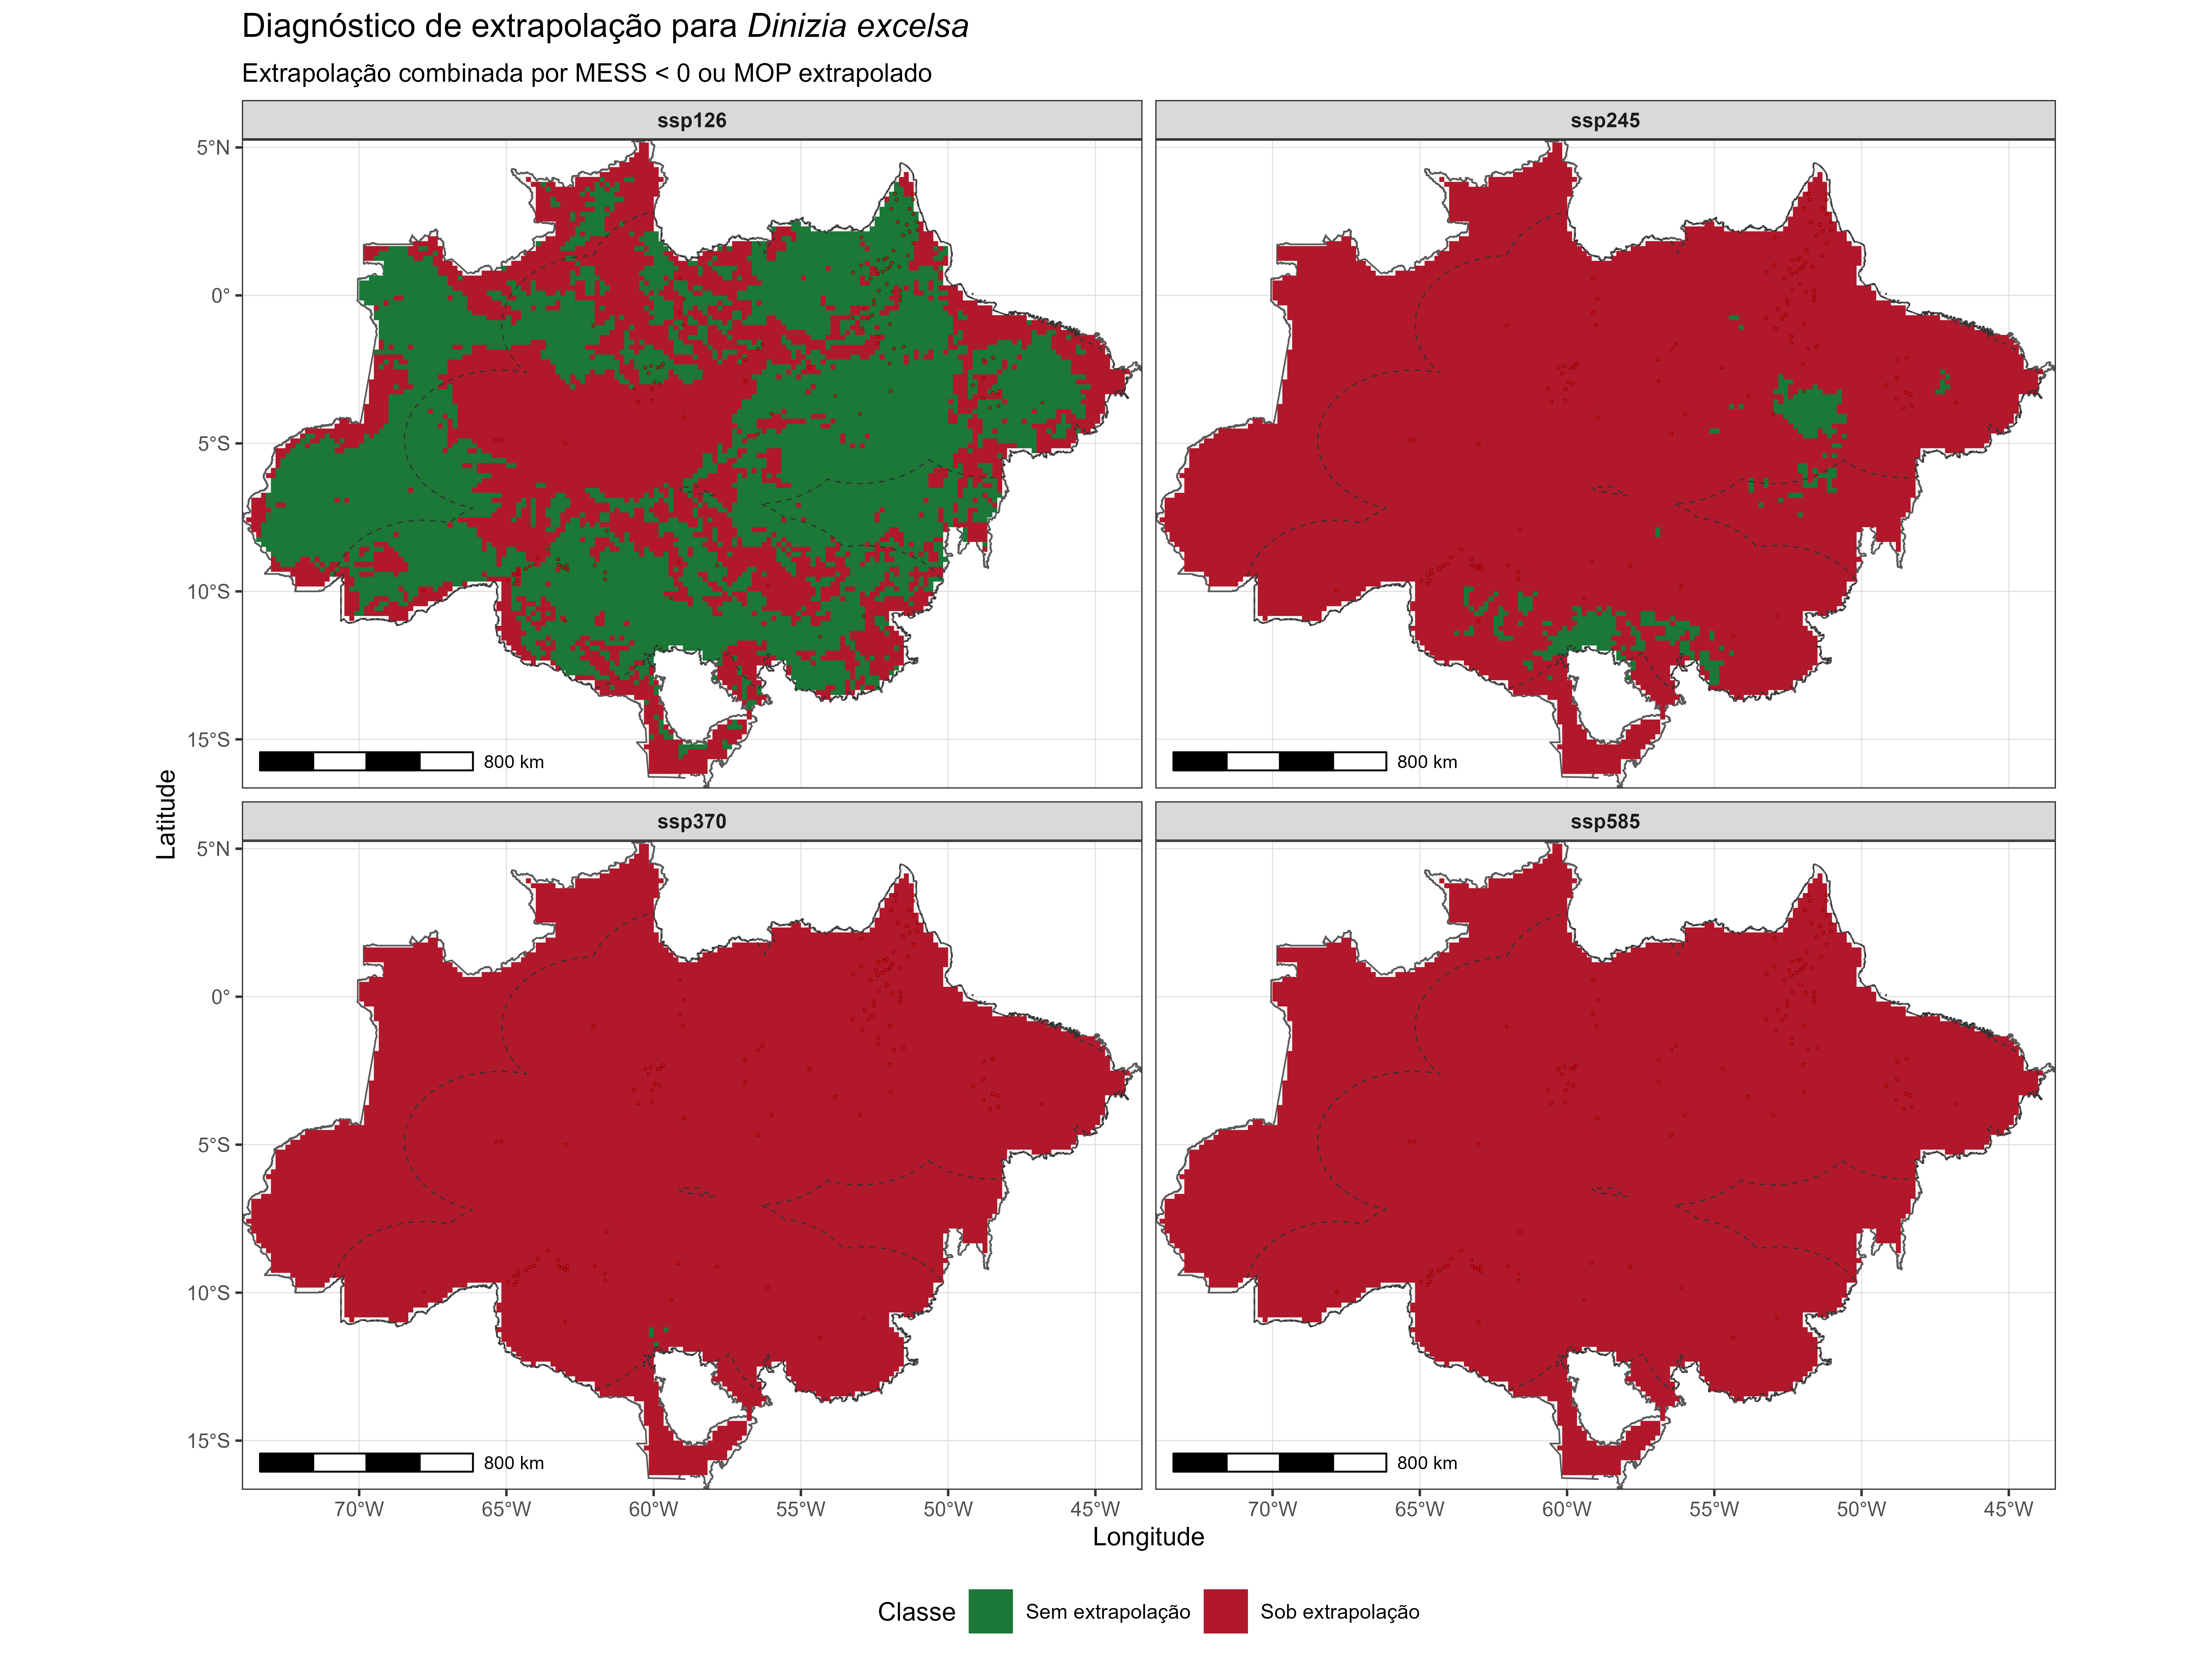
\includegraphics[width=0.96\textwidth]{figuras/unidade14/unidade14_adequabilidade_extrapolacao.png}
	\caption{Adequabilidade futura combinada com diagnóstico de extrapolação ambiental.}
	\label{fig:unidade14_adequabilidade_extrapolacao}
\end{figure}

\section{Síntese da extrapolação}

\rscriptfile{scripts/unidade14/06_sintese_extrapolacao.R}

\begin{figure}[H]
	\centering
	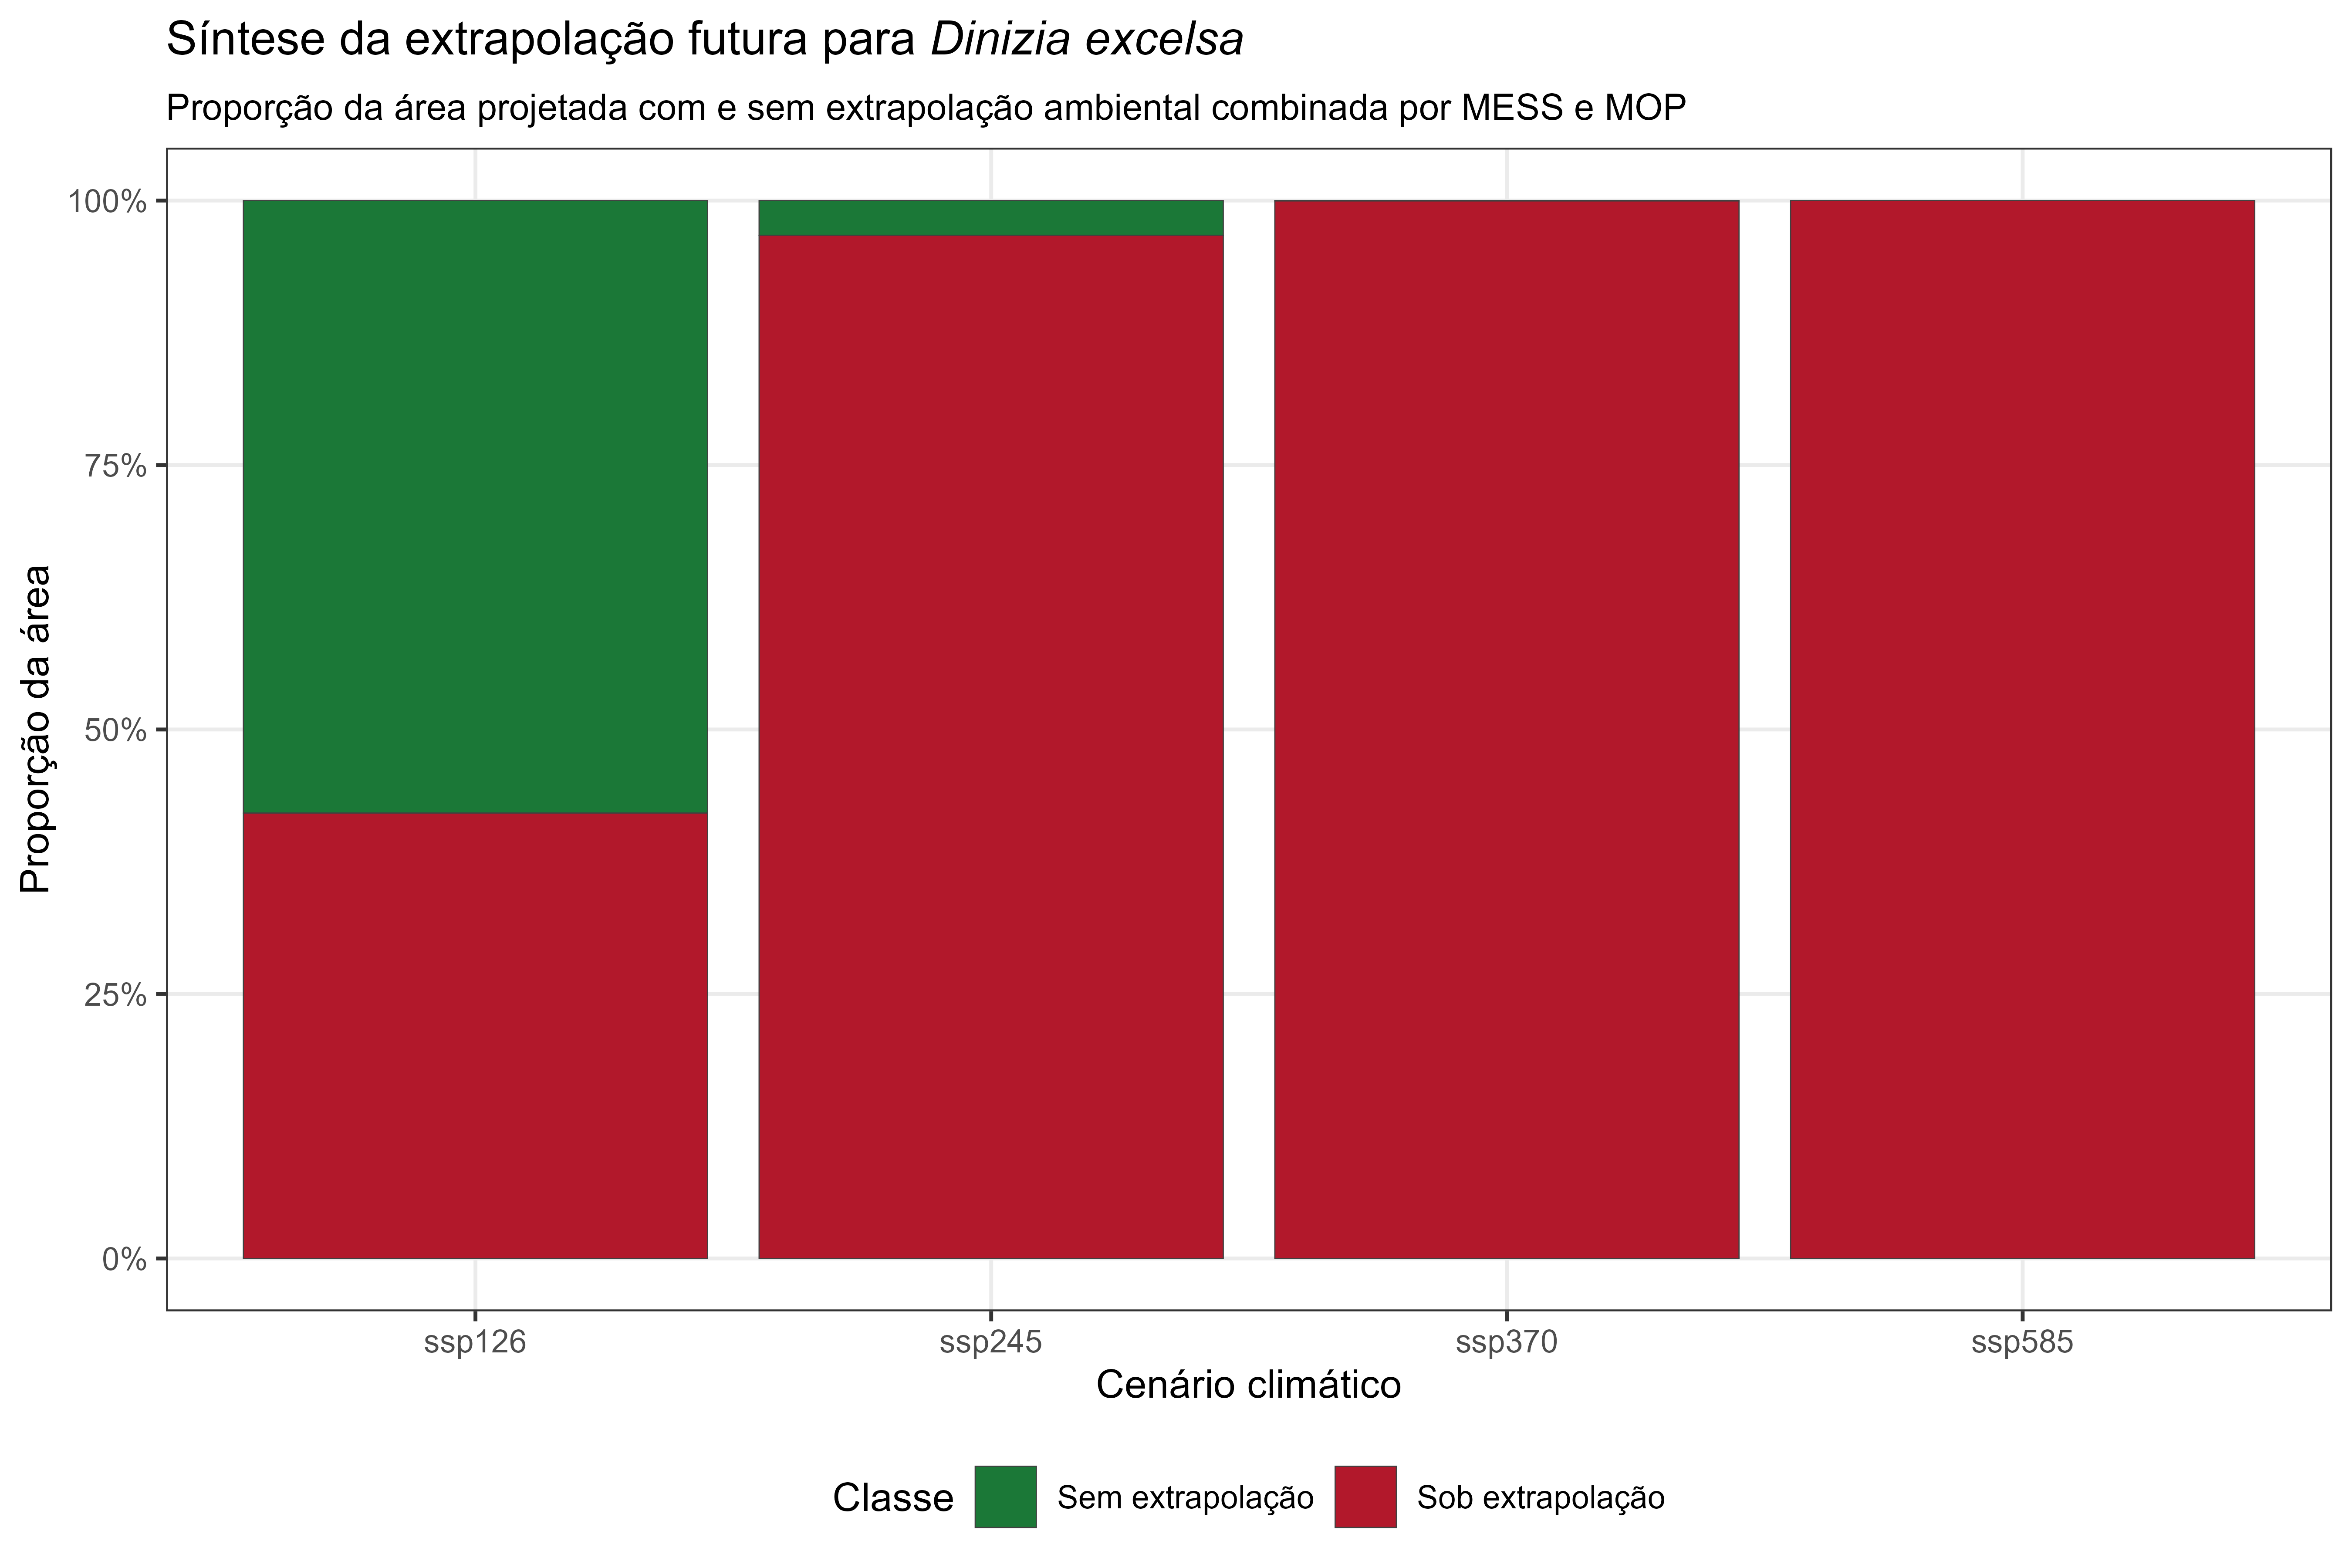
\includegraphics[width=0.88\textwidth]{figuras/unidade14/unidade14_sintese_extrapolacao.png}
	\caption{Proporção da área futura sob extrapolação ambiental em cada cenário SSP.}
	\label{fig:unidade14_sintese}
\end{figure}

\section{Pipeline completo}

\rscriptfile{scripts/unidade14/07_pipeline_transferencia_extrapolacao.R}

\section{Síntese da unidade}

A transferência espacial e temporal é essencial para aplicações de SDM em mudanças climáticas, mas exige diagnóstico rigoroso de extrapolação. Para \textit{Dinizia excelsa}, os mapas MESS e MOP permitem identificar regiões onde as projeções futuras devem ser interpretadas com maior cautela.

\begin{conceito}[title={\faBook\quad Mensagem central}]
	Projeções futuras só são ecologicamente defensáveis quando acompanhadas de diagnóstico de extrapolação. Áreas adequadas sob forte extrapolação devem ser interpretadas como hipóteses incertas, não como evidências robustas de persistência futura.
\end{conceito}

\section{Exercícios de fixação}

\begin{enumerate}
	\item Diferencie interpolação ambiental e extrapolação ambiental.
	\item Explique o que representa um valor negativo de MESS.
	\item Qual a diferença entre MESS e MOP?
	\item Por que modelos podem prever alta adequabilidade em áreas extrapolativas?
	\item Como mapas de extrapolação ajudam na interpretação de projeções futuras?
	\item Por que transferência temporal é especialmente sensível em cenários climáticos futuros?
	\item Como você usaria MESS e MOP para selecionar áreas prioritárias de conservação?
\end{enumerate}


% ============================================================
% UNIDADE 15
% ============================================================

